\documentclass{article}
\usepackage{graphicx} % Required for inserting images
\usepackage{amsmath}
\usepackage{booktabs}
\usepackage{amssymb}
\usepackage{hyperref}

\title{cdmo}
\author{
  Cirone Cono, \texttt{first1.last1@xxxxx.com}
  \and
  Dardini Jacopo, \texttt{first2.last2@xxxxx.com}
  \and
  Formichella Gio, \texttt{gio.formichella@studio.unibo.it}
  \and
  Petrozziello Giulio, \texttt{first2.last2@xxxxx.com}
}
\date{}

\begin{document}

\maketitle

\section{Introduction}
In this project we tackle the sport scheduling problem with CP, SAT, SMT and MIP, and apply with all 4 technologies the common approach described in \cite{10.1007/10704567_6}. All implementations take as input the number of teams in the tournament and start by precomputing the weekly matchups for the round-robin tournament; the matchups are stored in a matrix indexed by weeks and periods. The precomputation cost is minimal, for all tested team sizes the precomputation required less than a second. The matchup matrix not only speeds up the search by reducing the problem to ordering matchups, but also guarantees that the constraints of each team playing each other and playing once a week are satisfied. With all four techniques, we aim to find a solution satisfying the constraints and minimizing the objective variable D, the maximum difference between games played at home and away for a team; $D\in [1, n-1]$, where n is the number of teams. 

\section{CP Model}
\subsection{Decision Variables}
This model utilizes two primary decision variables to construct the tournament schedule and assign home/away teams for each match.

\subsubsection{\text{matches}}
The variable $\text{matches}_{p, w} \in [0, \dots, \frac{N}{2} - 1]$ for $p \in P, w \in W$, determines which match from the predefined round-robin structure ($\text{rb}$) is scheduled in week $w$ and period $p$.

\subsubsection{\text{home\_away}}
The binary variable $\text{home\_away}_{p, w} \in \{0, 1\}$ for $p \in P, w \in W$, assigns the home team for the match scheduled at period $p$ in week $w$. Specifically, $\text{home\_away}_{p, w} = 0$ means the first team listed in the match plays at home, while $\text{home\_away}_{p, w} = 1$ means the second team plays at home.

\subsection{Auxiliary Variables}
\subsubsection{\text{home\_games}}
The auxiliary variable $\text{home\_games}_{t} \in [1, \dots, N-1]$ for $t \in T$, represents the total number of home games assigned to team $t$ throughout the tournament. Its value is derived from the assignments of the decision variables $\text{matches}$ and $\text{home\_away}$.


\subsection{Objective Function}

The model's objective is to quantify and minimize disparities in home game assignments through the $\text{max\_imbalance}$ variable.

\subsubsection{Objective Variable: \text{max\_imbalance}}\label{objective}
The integer variable $\text{max\_imbalance} \in [1, \dots, N-1]$ quantifies the maximum absolute disparity in home game assignments across all teams. The lower bound of 1 acknowledges that perfect balance ($\text{max\_imbalance}=0$) is not achievable for an odd number of total games ($N-1$ games). The upper bound of $N-1$ represents the theoretical maximum possible deviation, occurring if a team plays all its games either at home or away.

The value of $\text{max\_imbalance}$ is determined by the following fairness constraint:
\[ \forall t \in T : \left| 2 \times \text{home\_games}_{t} - (N-1) \right| \leq \text{max\_imbalance} \]
This formulation precisely defines the absolute "imbalance" for each team $t$. This imbalance is derived from the difference between a team's home games and away games. Since $\text{home\_games}_{t} + \text{away\_games}_{t} = N-1$ (total games), substituting the expression for $\text{away\_games}_{t}$ yields the imbalance for team $t$ as $2 \times \text{home\_games}_{t} - (N-1)$. By enforcing that the absolute value of this imbalance for every team must be less than or equal to $\text{max\_imbalance}$, this variable effectively captures the largest such deviation among all teams, serving as the direct measure of the overall schedule's fairness.


\subsubsection{Objective}
The objective is to \textbf{minimize $\text{max\_imbalance}$}:
\[ \text{minimize } \text{max\_imbalance} \]
This aims to achieve the fairest possible distribution of home and away games. An optimal solution would ideally yield $\text{max\_imbalance}=1$, meaning each team's home/away game count differs by at most one, which is the best possible outcome for an odd number of total games played.


\subsection{Constraints}
\subsubsection{Core Constraints}
These constraints are strictly necessary for defining a feasible round-robin schedule:
\begin{enumerate}
    \item \textbf{Each period must be used exactly once per week:} Ensures that for every week, all matches generated by the round-robin structure's periods are indeed scheduled. Without this, some pairings might be missed, or periods might be duplicated, leading to an incomplete or invalid schedule.
    \[ \forall w \in W : \texttt{all\_different}([\texttt{matches}[p, w] \mid p \in P]) \]

    \item \textbf{Each team plays at most twice per period:} 
\[ \forall p \in P, \forall t \in T : \left| \{ (w, s) \mid w \in W, s \in S, \text{rb}_{\text{matches}_{p, w}, w, s} = t \} \right| \leq 2 \]

 \item \textbf{Calculation of Home Games:} This constraint defines the value of $\text{home\_games}_{t}$.
\[ \forall t \in T : \text{home\_games}_{t} = \sum_{p \in P, w \in W, s \in S} \mathbb{I}\left( \text{rb}_{\text{matches}_{p, w}, w, s} = t \land \text{home\_away}_{p, w} = s \right) \]
The indicator function $\mathbb{I}(\cdot)$ ensures that 1 is added to the sum if team $t$ is located in slot $s$ and that slot $s$ is designated as the home slot by $\text{home\_away}_{p,w}$.



    \item \textbf{Fairness - balance home and away games:} This constraint directly links the calculated $\text{home\_games}$ for each team to the objective variable $\text{max\_imbalance}$. For a detailed explanation of this relationship and the definition of $\text{max\_imbalance}$, please refer to Section \ref{objective} (Objective Variable and Objective Function).
    
    
\end{enumerate}

\subsubsection{Implied Constraints}

\begin{enumerate}
    \item \textbf{Each team appears exactly once per week:}
    \[ \forall w \in W, \forall t \in T : \left| \{ (p, s) \mid p \in P, s \in S, \text{rb}_{\text{matches}_{p, w}, w, s} = t \} \right| = 1 \]
\end{enumerate}

\subsubsection{Symmetry Breaking Constraints}

\begin{enumerate}
    \item \textbf{Break period assignment symmetry using lexicographic ordering:} The order in which matches corresponding to $P$ are assigned within $\text{matches}$ for each week is symmetrical. This constraint breaks such symmetries by enforcing a lexicographical ordering, reducing the number of equivalent search paths.
    \[ (\text{matches}_{p, w})_{p \in P, w \in W} \succeq_{\text{lex}} (\text{matches}_{p, w})_{\text{reversed}(p) \in P, w \in W} \]
    This states that the sequence of $\text{matches}$ variables, when read in normal $(p,w)$ order, must be lexicographically greater than or equal to when read in $(p,w)$ order with $p$ reversed. This helps to fix one permutation of period assignments.

    \item \textbf{Fix first match home assignment to break home/away symmetry:} This constraint eliminates global home/away assignment symmetry by fixing the home/away status of the first match.
    \[ \text{home\_away}_{0, 0} = 0 \]

\item \textbf{Balance the home/away assignments within each week:} While not a strict symmetry breaking constraint, this constraint helps reduce the search space by ensuring that within each week $w$, the number of matches where the second team plays at home ($\text{home\_away}_{p, w}=1$) is roughly half of the total matches ($|P|$), with a maximum deviation of 1:
\[ \forall w \in W : \left| \sum_{p \in P} \text{home\_away}_{p, w} - \left\lfloor \frac{|P|}{2} \right\rfloor \right| \leq 1 \]
This guides the solver towards balanced assignments and prunes highly imbalanced weekly configurations.

\end{enumerate}

\subsection{Validation}

The model was implemented in MiniZinc and validated through a series of experiments designed to assess solver performance under various model configurations and search strategies.

\subsubsection{Experimental Design}

To comprehensively evaluate the performance of different solving strategies for the Sports Tournament Scheduling problem, a systematic experimental study was conducted.

\textbf{Hardware and Software:}
Experiments were executed on a MacBook Air M1 equipped with an 8-core CPU. The following solvers were employed: \textit{Gecode}, \textit{Chuffed} and \textit{OR-Tools CP-SAT}. 
A uniform time limit of $300$ seconds was imposed for each individual problem instance.

\textbf{Model Configurations:}
Four configurations were tested: \texttt{baseline (core)}, \texttt{baseline+implied}, \texttt{baseline+symmetry breaking}, \texttt{full model}.

\textbf{Search Strategies:}
Three distinct search strategies were employed to analyze solver behavior, with a particular focus on how they influenced Gecode, often considered to have weaker default heuristics compared to modern SAT-based solvers.

\textbf{Search Strategies:}
Three distinct search strategies were employed to analyze solver behavior, focusing on their influence on Gecode, given its often weaker default heuristics compared to modern SAT-based solvers.

\begin{enumerate}
    \item \textbf{Default Search Strategy (Solver's Default):} Each solver relied entirely on its built-in decision heuristics and restart policies, serving as a baseline for their inherent capabilities.

    \item \textbf{Sequential Custom Search Strategy:} A manually defined sequential search (\texttt{seq\_search}) was applied, prioritizing \texttt{matches} variables with \texttt{dom\_w\_deg} and \texttt{home\_away} variables with \texttt{first\_fail}, utilizing a \texttt{restart\_luby(100)} policy.

    \item \textbf{Relax-and-Reconstruct (LNS) Strategy:} This higher-level strategy incorporated \texttt{relax\_and\_reconstruct} on the \texttt{matches} variables (preserving 60\% of solution values), leveraging Large Neighborhood Search (LNS) techniques. It was layered on top of the "Sequential Custom Search Strategy."
\end{enumerate}

\textbf{Solver-Specific Strategy Application:}
To ensure a fair and controlled comparison under single-threaded conditions (aligning with project constraints), OR-Tools CP-SAT was run without multi-threading. For both Chuffed and OR-Tools CP-SAT, the \texttt{free\_search} parameter was explicitly omitted when applying the custom Sequential Custom Search and Relax-and-Reconstruct strategies. This allowed direct evaluation of the user-defined MiniZinc search annotations, rather than the solvers' highly optimized default heuristics.


\subsubsection{Experimental Results}
\begin{table}[htbp]
\centering
\small
\resizebox{\textwidth}{!}{%
\begin{tabular}{c|cccc|cccc|cccc}
\toprule
\textbf{n} & \multicolumn{4}{c|}{\textbf{GECODE}} & \multicolumn{4}{c|}{\textbf{CHUFFED}} & \multicolumn{4}{c}{\textbf{CP-SAT}} \\
\cmidrule(lr){2-5}\cmidrule(lr){6-9}\cmidrule(lr){10-13}
  & bs & complete & noIMPL & noSB & bs & complete & noIMPL & noSB & bs & complete & noIMPL & noSB \\
\midrule
6 & 0 & 0 & 0 & 0 & 0 & 0 & 0 & 0 & 0 & 0 & 0 & 0 \\
8 & 6 & 6 & 6 & 6 & 0 & 0 & 0 & 0 & 0 & 0 & 0 & 0 \\
10 & N/A & N/A & N/A & N/A & 0 & 0 & 0 & 0 & 1 & 1 & 1 & 1 \\
12 & N/A & N/A & N/A & N/A & 60 & 6 & 5 & 6 & 4 & 3 & 3 & 3 \\
14 & N/A & N/A & N/A & N/A & 175 & 175 & 180 & 194 & 5 & 5 & 5 & 5 \\
16 & N/A & N/A & N/A & N/A & N/A & N/A & N/A & N/A & 15 & 15 & 15 & 15 \\
18 & N/A & N/A & N/A & N/A & N/A & N/A & N/A & N/A & 273 & 265 & 265 & 265 \\
20 & N/A & N/A & N/A & N/A & N/A & N/A & N/A & N/A & 85 & 84 & 84 & 84 \\
22 & N/A & N/A & N/A & N/A & N/A & N/A & N/A & N/A & 239 & 226 & 247 & 218 \\
\bottomrule
\end{tabular}%
}
\caption{CPU time in seconds for finding the \textit{optimal solution} using \textit{Default Search Strategy (Solver's Default)}}
\end{table}

\begin{table}[htbp]
\centering
\small
\resizebox{\textwidth}{!}{%
\begin{tabular}{c|cccc|cccc|cccc}
\toprule
\textbf{n} & \multicolumn{4}{c|}{\textbf{GECODE}} & \multicolumn{4}{c|}{\textbf{CHUFFED}} & \multicolumn{4}{c}{\textbf{CP-SAT}} \\
\cmidrule(lr){2-5}\cmidrule(lr){6-9}\cmidrule(lr){10-13}
  & bs & complete & noIMPL & noSB & bs & complete & noIMPL & noSB & bs & complete & noIMPL & noSB \\
\midrule
6 & 0 & 0 & 0 & 0 & 0 & 0 & 0 & 0 & 0 & 0 & 0 & 0 \\
8 & 0 & 0 & 0 & 0 & 0 & 0 & 0 & 0 & 0 & 0 & 0 & 0 \\
10 & 0 & 0 & 0 & 0 & 0 & 0 & 0 & 0 & 1 & 1 & 1 & 1 \\
12 & 0 & 0 & 0 & 0 & 0 & 0 & 0 & 0 & 55 & 56 & 58 & 48 \\
14 & 4 & 7 & 4 & 7 & N/A & 53 & 34 & N/A & N/A & N/A & N/A & N/A \\
16 & N/A & N/A & 191 & 164 & N/A & N/A & N/A & N/A & N/A & N/A & N/A & N/A \\
\bottomrule
\end{tabular}%
}
\caption{CPU time in seconds for finding the \textit{optimal solution} using \textit{Sequential Custom Search Strategy}}
\end{table}

\begin{table}[htbp]
\centering
\small
\resizebox{\textwidth}{!}{%
\begin{tabular}{c|cccc|cccc|cccc}
\toprule
\textbf{n} & \multicolumn{4}{c|}{\textbf{GECODE}} & \multicolumn{4}{c|}{\textbf{CHUFFED}} & \multicolumn{4}{c}{\textbf{CP-SAT}} \\
\cmidrule(lr){2-5}\cmidrule(lr){6-9}\cmidrule(lr){10-13}
  & bs & complete & noIMPL & noSB & bs & complete & noIMPL & noSB & bs & complete & noIMPL & noSB \\
\midrule
6 & 0 & 0 & 0 & 0 & 0 & 0 & 0 & 0 & 0 & 0 & 0 & 0 \\
8 & 0 & 0 & 0 & 0 & 0 & 0 & 0 & 0 & 0 & 0 & 0 & 0 \\
10 & 0 & 0 & 0 & 0 & 0 & 0 & 0 & 0 & 1 & 1 & 1 & 1 \\
12 & 0 & 0 & 0 & 0 & 9 & 1 & 3 & 2 & 56 & 62 & 59 & 52 \\
14 & 1 & 5 & 1 & 0 & N/A & 89 & 187 & 258 & N/A & N/A & N/A & N/A \\
16 & 184 & 19 & 1 & 8 & N/A & N/A & N/A & N/A & N/A & N/A & N/A & N/A \\
18 & N/A & 3 & N/A & N/A & N/A & N/A & N/A & N/A & N/A & N/A & N/A & N/A \\
\bottomrule
\end{tabular}%
}
\caption{CPU time in seconds for finding the \textit{optimal solution} using \textit{Relax-and-Reconstruct (LNS) Strategy}}
\end{table}


\section{MIP}
\subsection{Decision variables}
\subsubsection{matches}
The binary decision variables $X_{wpm}$ are equal to 1 iff in week w and period p match m is played.

\subsubsection{slots}
The binary decision variables $A_{wp}$ determine which team plays at home and which away. A is indexed by weeks and periods, so $A_wp$ corresponds to the matchup between teams $t_1, t_2$ in week w and period p; if $A_{wp} = 0$ then $t_1$ plays at home and $t_2$ away, if, otherwise, $A_{wp} = 1$ the order is reversed.

\subsubsection{team periods of play}
The binary variables TP are used to constrain each team to playing at most twice in the same period. $TP_{twp} = 1$ iff team t plays in week w and period p. 

\subsubsection{home games counter}
To compute the common objective function in MIP, it is necessary to introduce an array of integer auxiliary variables H such that $H[t]$ is the number of home games team t plays, bounded in $[0, n-1]$.

\subsection{Objective variables}
To compute D as the maximum difference between games played at home and away for all teams, we first find for each team the number of games played at home (2), and then constraint D as being greater or equal than the difference of home and away games for each team, given that we have a minimization problem this is effectively equivalent to computing the max. The absolute value of the difference is not computed explicitly but decomposed into 2 inequalities (3)(4). Finally, we look for the minimum of D (1)

\begin{align}
    &\min  D \\
    H_t =& \sum_{w, p} (A_{wp} = 0 \land G_{wp}[\text{home}] = t) \notag \\
    +& \sum_{w, p} (A_{wp} = 1 \land G_{wp}[\text{away}] = t) \hspace{20px}  &&t =1, \dots, n\\
    D &\geq 2H_t - (n-1) && t = 1, \dots, n\\
    D & \geq -(2 H_t - (n-1)) && t = 1, \dots, n
\end{align}


\subsection{Constraints}
\subsubsection{periods and matches}
Due to how the decision variables are defined, it was necessary to impose that each period in each week is assigned a single match (5) and each match is assigned to a single period (6).

\begin{align}
    \sum_{m = 1}^{n/2} X_{wpm} &= 1 \hspace{20px} p =1, \dots, n/2 \hspace{10px} w = 1,\dots, n-1 \\
    \sum_{p = 1}^{n/2} X_{wpm} &= 1 \hspace{20px} m = 1, \dots, n/2 \hspace{10px} w = 1,\dots, n-1
\end{align}

\subsubsection{team playing at most twice in the same period}
The constraint on teams playing at most twice in the same period was imposed by first linking the variables of X to those in TP based on the values in G (7) and then imposing that the sum of periods of play is smaller than 2 (8). 

\begin{align}
    TP_{twp} &= X_{wpm} \hspace{20px} G_{wm} =(t1, t2) \land (t = t1 \lor t=t2) \hspace{20px} \forall t \forall p  \forall w\\
    \sum_{w=1}^{n-1} &TP_{twp} \leq 2 \hspace{40px} t=1, \dots, n \hspace{10px} p = 1, \dots, n/2
\end{align}

\subsection{Validation}
\subsubsection*{Experimental design}
The model was written in Python by making use of the PuLP library and the solvers tested on the MIP model were: CBC 2.10.3, HiGHS 1.10.0, CPLEX 22.1.1 and SCIP 5.5.0 with their default parameters. The time elapsed to find an optimal solution, within the 300 second time limit, was measured and results presented in Fig.\ref{fig:MIP-solution} . All tests were run on a single core of an Intel i7-10750H CPU.

\subsubsection*{Experimental results}
As shown in Fig. \ref{fig:MIP-solution} CBC had the worst performance, it isn't able to find the optimal solution for n greater than 14. CPLEX, instead, was the fastest up to n=14 but after n=16 it stopped finding the optimal solution. HiGHS was able to find an optimal solution up to n=18 and SCIP, the best performer of the four, was able to reach n=20.

It was also verified that the solvers either found and optimal solution or no solution at all.

\begin{figure}
    \centering
    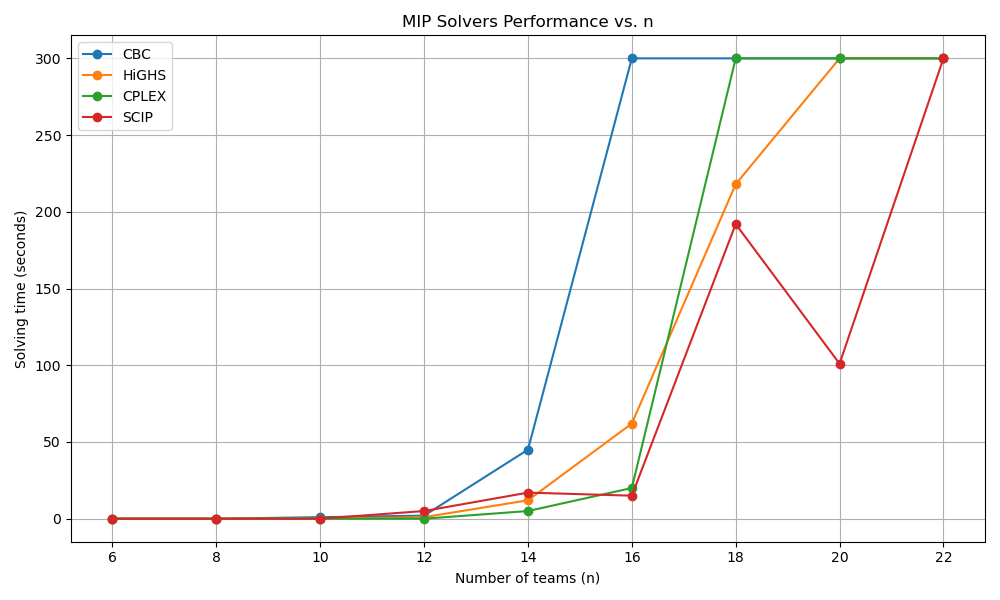
\includegraphics[width=0.8\linewidth]{img/MIP-result.png}
    \caption{MIP optimization}
    \label{fig:MIP-solution}
\end{figure}

\bibliographystyle{unsrt}
\bibliography{ref.bib}

\end{document}
